\documentclass[11pt]{article}

\usepackage[margin=1in]{geometry}
\usepackage{graphicx}
\usepackage{amsmath, amssymb, amsthm}
\usepackage{booktabs}
\usepackage{xcolor}
\usepackage{hyperref}
\usepackage{caption}
\usepackage{subcaption}
\usepackage{algorithm}
\usepackage{algpseudocode}
\usepackage{enumitem}

\hypersetup{
  colorlinks=true,
  linkcolor=black,
  citecolor=blue,
  urlcolor=blue
}

\newcommand{\Otilde}{\tilde{\mathcal{O}}}
\newcommand{\R}{\mathbb{R}}
\newcommand{\E}{\mathbb{E}}

\title{\vspace{-2em}\textbf{RLHF with Active Queries:\\Query-Efficient Alignment via Active Learning}\\[6pt]
\large A reading and replication report on Ji, He, Gu (2025)}
\author{Qiankun Li \quad Son Noel\\IE6520 --- Group 6}
\date{}

\begin{document}
\maketitle
\vspace{-2em}

\begin{abstract}
\noindent
We report on the paper \emph{Reinforcement Learning from Human Feedback with Active Queries}~\cite{jiheGu}, which studies RLHF as a contextual dueling bandit and proposes two algorithms: APPO, a theoretical algorithm with $\Otilde(d^2/\Delta)$ regret and $\Otilde(d^2/\Delta^2)$ query complexity, both independent of the action space size, and ADPO, a practical adaptation to direct preference optimisation~\cite{rafailov} that reaches or exceeds DPO's performance while using at most half the human labels. We walk through the problem formulation, the algorithm, the proof sketch, and the paper's experiments, then we run our own replication on a synthetic Bradley--Terry benchmark and three stress tests intended to find where the method breaks. We also respond to the feedback we received after our presentation: whether $\Delta$ depends on unknown parameters, what principled choices exist for the threshold, and where the pseudo-label idea can be pushed further.
\end{abstract}

\section{Introduction}

RLHF is the alignment recipe behind every recent open-weights chat model, and the bottleneck is the same in every implementation: pairs of model outputs go to human annotators, and a reward model (or the language model itself, in DPO~\cite{rafailov}) is trained on the resulting preferences. Figure~\ref{fig:rlhf} shows what the annotator sees. The reward signal then drives either a policy-gradient inner loop (PPO) or, in DPO's case, a supervised loss directly on the language-model parameters. Either way, human labels are the bottleneck: they are slow, expensive, and noisy near the decision boundary.

\begin{figure}[h]
  \centering
  \includegraphics[width=0.85\linewidth]{ss1.png}
  \caption{A typical RLHF preference interface. The annotator picks the better of two responses and the preference is used as a reward signal.}
  \label{fig:rlhf}
\end{figure}

The natural question is whether we need to query the annotator on \emph{every} preference pair, or whether a model that already has a clear view on a pair can just answer for itself. Ji, He and Gu formalise this as a linear contextual dueling bandit with an active-query rule and give a theoretical analysis with matching regret and query complexity bounds. Both bounds are \emph{constant in $T$} and \emph{independent of $|\mathcal{A}|$}, which is the part that had not been achieved in previous work.

This report has three aims. We walk through the theory carefully enough that a reader who has not opened the paper can follow the argument. We then replicate the practical algorithm (ADPO) on a small synthetic benchmark and on three stress settings we designed to find failure modes. Finally, we respond in writing to the feedback from Professor Wang Chi following our presentation, especially whether $\Delta$ itself depends on unknown parameters and how one might set the threshold in a more principled way.

\section{Problem setup: contextual dueling bandits}

The RLHF training loop fits neatly into the contextual dueling bandit template. At each round $t = 1, 2, \dots, T$,
\begin{enumerate}[leftmargin=*,itemsep=1pt]
  \item the environment draws a context $x_t \sim \mathcal{D}$ from a context space $\mathcal{X}$;
  \item the learner picks two actions $y_t^1, y_t^2 \in \mathcal{A}$ (in RLHF, two model responses);
  \item the annotator returns a preference $o_t \in \{0, 1\}$ whose distribution is
  \[
    \mathbb{P}(o_t = 1 \mid x_t, y_t^1, y_t^2)
    = \sigma\bigl(r(x_t, y_t^1) - r(x_t, y_t^2)\bigr),
    \qquad \sigma(z) = \frac{1}{1 + e^{-z}}.
  \]
\end{enumerate}
So the preference is a Bradley--Terry coin flip: a larger reward gap shifts the probability towards the better action, and when the two actions are tied the annotator is maximally unsure. The reward model is linear,
\[
  r(x, y) = \langle \theta^*, \phi(x, y) \rangle,
  \qquad \theta^* \in \R^d,\ \|\theta^*\|_2 \le B,\ \|\phi(x, y)\|_2 \le L/2.
\]
We pick one of the two actions, call it $y_t^1$, as the action whose quality actually counts, and measure the cumulative regret
\[
  \mathrm{Regret}(T) = \sum_{t=1}^T \bigl( r^*(x_t) - r(x_t, y_t^1) \bigr),
  \qquad r^*(x_t) = \max_{y \in \mathcal{A}} r(x_t, y).
\]
The paper assumes a \emph{minimum reward gap} $\Delta > 0$: on any context $x$, the optimal action is strictly better than every other action by at least $\Delta$. This is the single assumption on which the whole theory rests, and it is the object of the professor's feedback --- we return to it in Section~\ref{sec:delta}.

\paragraph{An informal example.}
It sometimes helps to think about movie recommendation rather than LLMs. The context is the user: age, genre preferences, recent viewing history. The action space is the library of movies. At each round the system shows two movies, the user picks one, and the system updates its estimate of which feature directions matter. The two formulations are mathematically the same; RLHF just has a much richer action space.

\section{The gap in prior work}

Earlier attempts at query-efficient RLHF split into two families.

\paragraph{Query-efficient but only randomised.}
\cite{zhan} and \cite{wangPO} produce $\varepsilon$-optimal randomised policies with $\Otilde(d^2 / \varepsilon^2)$ queries. The guarantee is on the expected sub-optimality of the randomised policy, not on a per-round regret, and these analyses cannot give an instance-dependent bound because the reward gap $\Delta$ does not appear anywhere.

\paragraph{Regret bounds but no query savings.}
\cite{wuSun} give a cumulative regret bound of $\Otilde(d^3 \sqrt{T})$, but the algorithm queries on every round, so the query count also grows linearly with $T$.

\paragraph{Instance-dependent but action-space-dependent.}
\cite{sekhari} do give an instance-dependent regret bound of $\Otilde(|\mathcal{A}|^2 d / \Delta)$ with $\Otilde(|\mathcal{A}|^3 d^2 / \Delta^2)$ queries. The $|\mathcal{A}|^2$ and $|\mathcal{A}|^3$ factors are the issue: in RLHF the action space is the set of plausible completions, so $|\mathcal{A}|$ is astronomical.

\paragraph{Direct preference optimisation.}
On the practical side, \cite{rafailov} observe that the reward model in RLHF can be folded into the language model itself, which removes the need for a separate reward-training phase and replaces the PPO inner loop with a supervised loss over preference pairs. DPO sets the scene for the present paper: the authors take DPO as their baseline and graft active querying on top of it.

The gap the paper fills is the intersection of these three strands --- an algorithm with simultaneously (i) an instance-dependent regret bound, (ii) a query budget that does not grow with $T$, and (iii) complexity that is independent of $|\mathcal{A}|$. Table~\ref{tab:comparison} summarises the comparison in one place.

\begin{table}[h]
  \centering\small
  \begin{tabular}{lccc}
    \toprule
    \textbf{Method} & \textbf{Regret} & \textbf{Query complexity} & $|\mathcal{A}|$-free? \\
    \midrule
    Zhan et al.\ (2023)     & $\Otilde(\sqrt{T})$ (worst-case only) & $\Otilde(d^2 / \varepsilon^2)$ & \checkmark \\
    Wu \& Sun (2023)        & $\Otilde(d^3 \sqrt{T})$ & linear in $T$ & \checkmark \\
    Sekhari et al.\ (2024)  & $\Otilde(|\mathcal{A}|^2 d / \Delta)$ & $\Otilde(|\mathcal{A}|^3 d^2 / \Delta^2)$ & $\times$ \\
    \textbf{APPO} (this paper) & $\Otilde(d^2 / \Delta)$ & $\Otilde(d^2 / \Delta^2)$ & \checkmark \\
    \bottomrule
  \end{tabular}
  \caption{Regret and query-complexity comparison across prior work and the paper's APPO algorithm. APPO is the first to be simultaneously instance-dependent, $T$-free, and $|\mathcal{A}|$-free.}
  \label{tab:comparison}
\end{table}

\paragraph{What the asymptotic differences mean numerically.}
The bounds in Table~\ref{tab:comparison} hide constants and logs, so the size of the improvement is not visible until one plugs in plausible RLHF numbers. Take a small reward head with $d = 10^3$ feature dimensions, a one-epoch training pass over a $T = 10^6$-pair dataset, an action set of $|\mathcal{A}| = 10^4$ candidate completions per prompt, and the gap reported in the paper's footnote, $\Delta = 0.5$ on the Ultrafeedback-binarised data. Then:
\begin{itemize}[leftmargin=*,itemsep=1pt]
  \item Wu \& Sun (2023): $\Otilde(d^3\sqrt{T}) \approx (10^3)^3 \cdot 10^3 = 10^{12}$.
  \item Sekhari et al.\ (2024): $\Otilde(|\mathcal{A}|^2 d / \Delta) \approx (10^4)^2 \cdot 10^3 / 0.5 \approx 2 \times 10^{11}$.
  \item APPO: $\Otilde(d^2 / \Delta) \approx (10^3)^2 / 0.5 \approx 2 \times 10^6$.
\end{itemize}
That is five to six orders of magnitude. The point of the comparison is not the exact number --- nobody runs RLHF in a regime where these regret bounds are tight --- but the asymptotic structure: at any horizon long enough to amortise the cost of training a reward model, the $T$-free and $|\mathcal{A}|$-free bound dominates. Both other bounds blow up before the action set reaches the size of a token vocabulary.

\section{The APPO algorithm}

The algorithm is reproduced in Figure~\ref{fig:appo}. At each round the learner maintains an estimate $\hat\theta_t$ of the reward parameter and uses an uncertainty check to decide whether to query the annotator. We unpack the three moving parts below.

\begin{figure}[h]
  \centering
  \includegraphics[width=0.95\linewidth]{APPO.png}
  \caption{APPO pseudocode (Algorithm~1 in the paper). The $\Gamma$-threshold check on line~6 is what makes the algorithm active; the policy update on line~11 is the exponential-weights rule from OPPO.}
  \label{fig:appo}
\end{figure}

\paragraph{(1) Regularised MLE on queried rounds only.}
Let $C_{t-1}$ be the set of rounds in which the annotator was queried before round $t$. The estimator $\hat\theta_t$ is defined as the solution of
\[
  \lambda \theta + \sum_{\tau \in C_{t-1}}
  \bigl[ o_\tau - \sigma(\langle \theta,\, \phi_\tau^1 - \phi_\tau^2 \rangle) \bigr]
  (\phi_\tau^1 - \phi_\tau^2) = 0,
\]
which is the first-order condition of a regularised logistic MLE. Only queried rounds contribute to $\hat\theta_t$; skipped rounds are dropped entirely. The design matrix $\Sigma_t = \lambda I + \sum_{\tau \in C_t} (\phi_\tau^1 - \phi_\tau^2)(\phi_\tau^1 - \phi_\tau^2)^\top$ is used to build a confidence ellipsoid around $\hat\theta_t$: with probability at least $1 - \delta$,
$
  \|\theta^* - \hat\theta_t\|_{\Sigma_{t-1}} \le \beta
$
for an appropriate radius $\beta$.

\paragraph{(2) Optimistic reward-gap estimate.}
Given $\hat\theta_t$, the algorithm forms an upper-confidence estimate of the reward gap relative to the second action:
\[
  \hat D_t(x, y) = \min\!\Bigl\{
    \langle \hat\theta_t,\, \phi(x, y) - \phi_t^2 \rangle
    + \beta \cdot \|\phi(x, y) - \phi_t^2\|_{\Sigma_{t-1}^{-1}},
    \ 1
  \Bigr\}.
\]
On the confidence event, Cauchy--Schwarz gives $\hat D_t(x, y) \ge D_t(x, y)$, so the estimate is a valid upper bound on the true gap.

\paragraph{(3) Exponential-weights policy update (OPPO).}
The policy $\pi_t$ is updated in the standard mirror-descent form,
\[
  \pi_{t+1}(y \mid x) \propto \pi_t(y \mid x) \cdot \exp\!\bigl( \eta \hat D_t(y, x) \bigr),
\]
and only on queried rounds. Skipped rounds advance $t$ but leave $\pi_t$ and $\Sigma_t$ untouched.

\paragraph{The active-query rule.}
The algorithm picks $y_t^1 = \arg\max_y \hat D_t(x_t, y)$ as the ``best'' action and draws $y_t^2$ uniformly from $\mathcal{A}$ as a comparison. It then checks
\[
  \|\phi_t^1 - \phi_t^2\|_{\Sigma_{t-1}^{-1}}
  \quad \text{vs.} \quad
  \Gamma.
\]
If the quantity on the left is below $\Gamma$, the algorithm skips the query. Otherwise it asks the annotator and logs $t$ into $C_t$. The norm $\|\cdot\|_{\Sigma_{t-1}^{-1}}$ measures how much the current pair $(\phi_t^1 - \phi_t^2)$ points in a direction the estimator has not yet seen --- a standard elliptical-bandits quantity.

\paragraph{Why skipping is safe.}
If the uncertainty is below $\Gamma$ and the radius $\beta$ is calibrated so that $2 \beta \Gamma < \Delta$ (this is Lemma~E.3 in the paper), then the UCB bound gives
\[
  D_t(x_t, y_t^*) - D_t(x_t, y_t^1) \le 2\beta\Gamma < \Delta.
\]
By the minimum-gap assumption the only way for the gap to be strictly less than $\Delta$ is for it to be exactly $0$, so $y_t^1$ is already optimal. Skipping in this regime incurs no regret at all. This is where the $\Delta > 0$ assumption earns its keep.

\section{Theoretical guarantees}
\label{sec:theory}

The main theorem we will prove is the following.

\begin{quote}
\textbf{Theorem 5.1.} Pick the algorithm parameters $\lambda = B^{-2}$, $\Gamma = \kappa_\sigma \Delta / (2 \sqrt{d}\, \iota_1)$, $\eta = \sqrt{\Gamma^2 \log|\mathcal{A}| / (32 d \log(3LB\Gamma^{-1}))}$, and $\beta = \kappa_\sigma^{-1}(1 + 4\sqrt{d \iota_2} + \sqrt{2 d \iota_3})$, with logarithmic factors $\iota_1, \iota_2, \iota_3$ as in Lemma~\ref{lem:safe} below. Then with probability at least $1 - \delta$,
\[
  \mathrm{Regret}(T) = \Otilde\!\left(\frac{d^2}{\Delta}\right),
  \qquad
  \mathrm{Query}(T) = |C_T| = \Otilde\!\left(\frac{d^2}{\Delta^2}\right).
\]
\end{quote}

Both bounds are independent of the horizon $T$ and of the action-set size $|\mathcal{A}|$. The $T$-independence comes from a query-budget bound that does not grow with $T$; the $|\mathcal{A}|$-independence enters through the OPPO regret, which sees $\mathcal{A}$ only via $\log|\mathcal{A}|$.

We build the proof in five steps. We first bound the size of the queried set (Lemma~\ref{lem:query}); we then control the estimator (Lemma~\ref{lem:conf}) and use it to verify that the UCB estimator is optimistic (Lemma~\ref{lem:opt}) and that skipping is safe (Lemma~\ref{lem:safe}). The OPPO regret (Lemma~\ref{lem:oppo}) handles the policy-update error. Combining the four pieces gives the theorem.

\subsection{Notation and assumptions}

Write $\phi_t^j = \phi(x_t, y_t^j)$ for $j \in \{1, 2\}$, $C_t \subseteq [t]$ for the set of rounds queried up to time $t$, and $\Sigma_t = \lambda I + \sum_{\tau \in C_t} (\phi_\tau^1 - \phi_\tau^2)(\phi_\tau^1 - \phi_\tau^2)^\top$ for the design matrix. The reward-gap relative to the baseline action $y_t^2$ is $D_t(x, y) = \langle \theta^*, \phi(x, y) - \phi_t^2 \rangle$ and its UCB estimate is
\[
  \hat D_t(x, y) = \min\!\bigl\{ \langle \hat\theta_t, \phi(x, y) - \phi_t^2 \rangle + \beta \|\phi(x, y) - \phi_t^2\|_{\Sigma_{t-1}^{-1}},\ 1 \bigr\}.
\]

The two structural assumptions of the analysis are: \emph{(A1)} bounded features and parameters, $\|\phi(x, y)\|_2 \le L/2$ and $\|\theta^*\|_2 \le B$, with rewards normalised to $r(x, y) \in [0, 1]$; \emph{(A2)} the link function $\sigma$ is differentiable with $\dot\sigma \ge \kappa_\sigma > 0$ on its domain (for the standard logistic link, $\kappa_\sigma = 1/(4 \cosh^2(B L /2))$); and \emph{(A3)} a strictly positive minimum gap, $\Delta := \min_x \min_{y \neq y^*(x)} (r^*(x) - r(x, y)) > 0$. (A1) and (A2) are standard for generalised linear bandits; (A3) is the assumption that does most of the heavy lifting for the constant-$T$ guarantee, and we revisit it in Section~\ref{sec:delta}.

\subsection{Bounding the number of queries}

\begin{lemma}[Query upper bound; paper Lemma E.1]
\label{lem:query}
For any $0 < \Gamma \le 1$ and $\lambda = B^{-2}$, the queried set satisfies
\[
  |C_T| \le 16 d \Gamma^{-2} \log(3 L B \Gamma^{-1}).
\]
\end{lemma}

\begin{proof}
For every $\tau \in C_T$ the threshold check failed, so $\|\phi_\tau^1 - \phi_\tau^2\|_{\Sigma_{\tau-1}^{-1}} > \Gamma$. Since $0 \le \Gamma \le 1$, this gives
\begin{equation}
  \sum_{\tau \in C_T} \min\!\bigl\{1,\ \|\phi_\tau^1 - \phi_\tau^2\|_{\Sigma_{\tau-1}^{-1}}^2\bigr\}
  \ge |C_T| \cdot \Gamma^2.
  \label{eq:query-lb}
\end{equation}
The elliptical-potential lemma (Lemma~G.7 of the paper, originally Lemma~10 of Abbasi-Yadkori et al., 2011) gives the matching upper bound
\begin{equation}
  \sum_{\tau \in C_T} \min\!\bigl\{1,\ \|\phi_\tau^1 - \phi_\tau^2\|_{\Sigma_{\tau-1}^{-1}}^2\bigr\}
  \le 2d \log\!\left( \frac{\lambda d + |C_T| L^2}{\lambda d} \right).
  \label{eq:query-ub}
\end{equation}
Combining \eqref{eq:query-lb} and \eqref{eq:query-ub} and dividing by $\Gamma^2$,
\[
  \frac{\Gamma^2 |C_T|}{2d}
  \le \log\!\left( 1 + \frac{2 L^2}{\Gamma^2 \lambda} \cdot \frac{\Gamma^2 |C_T|}{2d} \right).
\]
With $\lambda = B^{-2}$ and $2L^2 B^2 \ge \Gamma^2$, the inequality $u \le \log(1 + a u)$ has solution $u \le \tfrac{2}{a}\log(\tfrac{2}{a}) + 1$, which after substitution and simplification gives the claimed bound; full algebra is in Appendix~F.1 of the paper.
\end{proof}

Plugging $\Gamma = \kappa_\sigma \Delta / (2 \sqrt{d}\, \iota_1)$ from the recipe of Theorem~5.1 turns Lemma~\ref{lem:query} into the claimed query complexity:
\[
  |C_T|
  \le \frac{64 d^2 \iota_1^2}{\kappa_\sigma^2 \Delta^2} \cdot \log(\cdot)
  = \Otilde\!\left( \frac{d^2}{\Delta^2} \right).
\]

\subsection{Confidence ellipsoid for $\hat\theta_t$}

\begin{lemma}[Confidence set; paper Lemma E.2]
\label{lem:conf}
With probability at least $1 - \delta$, for every $t \in [T]$,
\[
  \|\theta^* - \hat\theta_t\|_{\Sigma_{t-1}}
  \le \frac{1}{\kappa_\sigma}\!\left( \sqrt{\lambda} B + \sqrt{2 d \log\bigl((\lambda + |C_t| L^2 / d)/(\lambda \delta)\bigr)} \right)
  =: \beta.
\]
\end{lemma}

\begin{proof}
Define the population first-order operator and the noise vector
\[
  G_t(\theta) := \lambda \theta + \sum_{\tau \in C_{t-1}} \bigl[\sigma(\langle \theta, \phi_\tau^1 - \phi_\tau^2 \rangle) - \sigma(\langle \theta^*, \phi_\tau^1 - \phi_\tau^2 \rangle)\bigr](\phi_\tau^1 - \phi_\tau^2),
  \qquad
  \epsilon_\tau = o_\tau - \sigma(\langle \theta^*, \phi_\tau^1 - \phi_\tau^2 \rangle),
  \qquad
  Z_t = \sum_{\tau \in C_{t-1}} \epsilon_\tau (\phi_\tau^1 - \phi_\tau^2).
\]
The MLE first-order condition (4.1 in the paper) reads $\lambda \hat\theta_t + \sum_{\tau} [\sigma(\langle \hat\theta_t, \phi_\tau^1 - \phi_\tau^2\rangle) - o_\tau](\phi_\tau^1 - \phi_\tau^2) = 0$. Substituting the definition of $\epsilon_\tau$ in $o_\tau = \sigma(\langle \theta^*, \cdot\rangle) + \epsilon_\tau$ and rearranging,
\begin{equation}
  G_t(\hat\theta_t) = Z_t,
  \qquad
  G_t(\theta^*) = \lambda \theta^*,
  \qquad\Longrightarrow\qquad
  G_t(\hat\theta_t) - G_t(\theta^*) = Z_t - \lambda \theta^*.
  \label{eq:lem-conf-1}
\end{equation}
Since $\sigma$ is differentiable, the mean-value theorem gives, for some $\tilde\theta_t$ on the segment between $\hat\theta_t$ and $\theta^*$,
\begin{equation}
  G_t(\hat\theta_t) - G_t(\theta^*)
  = F(\tilde\theta_t)(\hat\theta_t - \theta^*),
  \qquad
  F(\tilde\theta_t) := \lambda I + \sum_{\tau \in C_{t-1}} \dot\sigma\!\bigl(\langle \tilde\theta_t, \phi_\tau^1 - \phi_\tau^2 \rangle\bigr)(\phi_\tau^1 - \phi_\tau^2)(\phi_\tau^1 - \phi_\tau^2)^\top.
  \label{eq:lem-conf-2}
\end{equation}
By Assumption~(A2), $\dot\sigma \ge \kappa_\sigma$ pointwise, so $F(\tilde\theta_t) \succeq \kappa_\sigma \Sigma_{t-1}$ in the Loewner order. Combining \eqref{eq:lem-conf-1}--\eqref{eq:lem-conf-2},
\begin{equation}
  (\hat\theta_t - \theta^*)^\top F(\tilde\theta_t)^\top \Sigma_{t-1} F(\tilde\theta_t) (\hat\theta_t - \theta^*)
  = \|Z_t - \lambda\theta^*\|_{\Sigma_{t-1}^{-1}}^2 \cdot \text{(constants)},
\end{equation}
and after standard inverse manipulation,
\[
  \|\hat\theta_t - \theta^*\|_{\Sigma_{t-1}}
  \le \kappa_\sigma^{-1} \|Z_t - \lambda\theta^*\|_{\Sigma_{t-1}^{-1}}
  \le \kappa_\sigma^{-1} \bigl(\|Z_t\|_{\Sigma_{t-1}^{-1}} + \sqrt{\lambda} B\bigr),
\]
using the triangle inequality and $\|\lambda\theta^*\|_{\Sigma_{t-1}^{-1}}^2 \le \lambda \|\theta^*\|_2^2 \le \lambda B^2$ since $\Sigma_{t-1} \succeq \lambda I$.

It remains to bound $\|Z_t\|_{\Sigma_{t-1}^{-1}}$. The sequence $\{\epsilon_\tau (\phi_\tau^1 - \phi_\tau^2)\}_\tau$ is a vector-valued martingale-difference sequence with respect to the filtration generated by the algorithm's history --- $\epsilon_\tau$ has zero conditional mean given the past by definition of $\sigma(\langle\theta^*, \cdot\rangle)$ as the conditional expectation of $o_\tau$ --- and each summand is bounded in $[-2, 2]$ in $\R$ along $\phi_\tau^1 - \phi_\tau^2$. The self-normalised concentration inequality of Abbasi-Yadkori, P\'al, Szepesv\'ari (2011, Theorem~1) then gives, for any fixed $\delta > 0$, with probability at least $1 - \delta$ uniformly over $t \in [T]$,
\begin{equation}
  \|Z_t\|_{\Sigma_{t-1}^{-1}}^2
  \le 2 \log\!\left( \frac{\sqrt{\det(\Sigma_{t-1})}}{\sqrt{\det(\Sigma_0)}\cdot \delta} \right).
  \label{eq:lem-conf-3}
\end{equation}
The determinant is bounded by the trace--AM-GM inequality $\det(\Sigma_{t-1})^{1/d} \le \mathrm{tr}(\Sigma_{t-1})/d$. Since $\mathrm{tr}(\Sigma_{t-1}) = d\lambda + \sum_{\tau \in C_{t-1}} \|\phi_\tau^1 - \phi_\tau^2\|_2^2 \le d\lambda + |C_t| L^2$,
\[
  \det(\Sigma_{t-1})
  \le \left( \lambda + \frac{|C_t| L^2}{d} \right)^d.
\]
With $\det(\Sigma_0) = \lambda^d$, plugging into \eqref{eq:lem-conf-3} yields
\[
  \|Z_t\|_{\Sigma_{t-1}^{-1}}
  \le \sqrt{2 d \log\!\left( \frac{\lambda + |C_t| L^2/d}{\lambda \delta} \right)}.
\]
Combining with the earlier bound on $\|\hat\theta_t - \theta^*\|_{\Sigma_{t-1}}$ produces $\beta$.
\end{proof}

For the parameters of Theorem~5.1, $\beta = \Otilde(\sqrt{d}/\kappa_\sigma)$.

\subsection{Optimism of the UCB estimator}

\begin{lemma}[UCB validity; paper Lemma E.4]
\label{lem:opt}
On the confidence event of Lemma~\ref{lem:conf}, for every $t \in [T]$, $x \in \mathcal{X}$ and $y \in \mathcal{A}$,
\[
  D_t(x, y) \le \hat D_t(x, y) \le D_t(x, y) + 2 \beta \|\phi(x, y) - \phi_t^2\|_{\Sigma_{t-1}^{-1}}.
\]
\end{lemma}

\begin{proof}
By Cauchy--Schwarz on the inner product and the confidence event,
\[
  |D_t(x, y) - \langle \hat\theta_t, \phi(x,y) - \phi_t^2 \rangle|
  = |\langle \hat\theta_t - \theta^*, \phi(x,y) - \phi_t^2 \rangle|
  \le \|\hat\theta_t - \theta^*\|_{\Sigma_{t-1}} \cdot \|\phi(x,y) - \phi_t^2\|_{\Sigma_{t-1}^{-1}}
  \le \beta \|\phi(x,y) - \phi_t^2\|_{\Sigma_{t-1}^{-1}}.
\]
Adding $\beta \|\phi(x,y) - \phi_t^2\|_{\Sigma_{t-1}^{-1}}$ to both sides of the resulting bound on $\langle\hat\theta_t, \phi-\phi_t^2\rangle - D_t \ge -\beta\|\cdots\|$ gives $\hat D_t \ge D_t$. The reverse direction adds the bonus a second time, yielding the upper bound.
\end{proof}

\subsection{Skipping is safe}

This is the central instance-dependent argument: on rounds where the threshold check fires, the UCB-chosen action is in fact optimal, not just close to optimal.

\begin{lemma}[Skipping safety; paper Lemma E.3]
\label{lem:safe}
Let $\iota_1 = 42 \log(126 L B \sqrt{d} \kappa_\sigma^{-1}) + \sqrt{8 \log(1/\delta)}$, $\iota_2 = \log(3 L B \Gamma^{-1})$, and $\iota_3 = \log\bigl((1 + 16 L^2 B^2 \Gamma^{-2} \iota_2)/\delta\bigr)$. With $\Gamma = \kappa_\sigma \Delta/(2\sqrt{d}\,\iota_1)$ and $\beta = \kappa_\sigma^{-1}(1 + 4\sqrt{d \iota_2} + \sqrt{2 d \iota_3})$,
\[
  2 \beta \Gamma < \Delta,
\]
and consequently every round $t \notin C_T$ contributes exactly $0$ to the regret.
\end{lemma}

\begin{proof}
The choice of $\beta$ satisfies the requirement of Lemma~\ref{lem:conf} on the confidence event (one verifies $\kappa_\sigma \beta \ge \sqrt{\lambda} B + \sqrt{2 d \log((\lambda + |C_T| L^2/d)/(\lambda \delta))}$ by plugging in $\lambda = B^{-2}$ and the bound on $|C_T|$ from Lemma~\ref{lem:query}; algebra in Appendix~F.3 of the paper). The inequality $2\beta\Gamma < \Delta$ follows by direct substitution and the calibration $\iota_1 \ge 2 + 4\sqrt{\iota_2} + \sqrt{2 \iota_3}$, which is what $\iota_1$ is designed to give.

For the second statement: on a non-queried round $t \notin C_T$, by definition of the algorithm $\|\phi_t^1 - \phi_t^2\|_{\Sigma_{t-1}^{-1}} \le \Gamma$. Apply Lemma~\ref{lem:opt} to the optimal action $y_t^*$ and to $y_t^1$:
\[
  D_t(x_t, y_t^*) - D_t(x_t, y_t^1)
  \le \bigl[\hat D_t(x_t, y_t^*) - \langle \theta^*, \phi(x_t, y_t^*) - \phi_t^2 \rangle\bigr]
    - 0
  \le 2 \beta \|\phi(x_t, y_t^*) - \phi_t^2\|_{\Sigma_{t-1}^{-1}}
\]
where we used $\hat D_t(x_t, y_t^*) \le \hat D_t(x_t, y_t^1)$ by the choice rule on Line~5 of Algorithm~1, plus Lemma~\ref{lem:opt}. The norm on the right is $\|\phi(x_t, y_t^*) - \phi_t^2\|_{\Sigma_{t-1}^{-1}} \le \|\phi_t^1 - \phi_t^2\|_{\Sigma_{t-1}^{-1}} \le \Gamma$ on a skipped round (using Lemma~E.4's chain in the paper for the first inequality), so
\[
  D_t(x_t, y_t^*) - D_t(x_t, y_t^1) \le 2 \beta \Gamma < \Delta.
\]
The minimum-gap assumption (A3) says the suboptimality is either $0$ or at least $\Delta$. The strict inequality forces it to be $0$.
\end{proof}

This is the lemma the entire constant-$T$ behaviour rests on. Without (A3) the inequality $2\beta\Gamma < \Delta$ would still hold but the gap could land anywhere in $(0, \Delta)$, leaving an $O(T)$ residual in the non-queried portion of the regret.

\subsection{OPPO regret on the queried subsequence}

\begin{lemma}[OPPO regret; paper Lemma E.5]
\label{lem:oppo}
Under the exponential-weights update $\pi_{t+1}(y \mid x) \propto \pi_t(y \mid x) \exp(\eta \hat D_t(y, x))$, applied only on rounds $t \in C_T$,
\[
  \E_{x \sim \mathcal{D}, y \sim \pi^*(\cdot \mid x)} [\hat D_t(x, y)]
  - \E_{x \sim \mathcal{D}, y \sim \pi_t(\cdot \mid x)} [\hat D_t(x, y)]
  \le 2\eta + \eta^{-1} \E_{x \sim \mathcal{D}}\bigl[ \mathrm{KL}(\pi^*(\cdot \mid x) \| \pi_t(\cdot \mid x)) - \mathrm{KL}(\pi^*(\cdot \mid x) \| \pi_{t+1}(\cdot \mid x)) \bigr].
\]
\end{lemma}

\begin{proof}
Fix a context $x$ and write $D := \hat D_t(x, \cdot)$, $\pi := \pi_t(\cdot \mid x)$, $\pi' := \pi_{t+1}(\cdot \mid x)$, $\pi^* := \pi^*(\cdot \mid x)$ to lighten notation. The exponential update can be rearranged into a per-action identity. By definition $\pi'(y) = \pi(y) \exp(\eta D(y)) / \rho$ with $\rho := \sum_y \pi(y) \exp(\eta D(y))$ a normaliser independent of $y$, so
\begin{equation}
  \eta D(y) = \log \pi'(y) - \log \pi(y) + \log \rho.
  \label{eq:lemoppo-1}
\end{equation}
Multiply both sides of \eqref{eq:lemoppo-1} by $(\pi^*(y) - \pi'(y))$ and sum over $y$. Because $\sum_y (\pi^*(y) - \pi'(y)) = 1 - 1 = 0$, the $\log\rho$ term drops out, leaving
\begin{equation}
  \eta \sum_y D(y)(\pi^*(y) - \pi'(y))
  = \sum_y \bigl(\log \pi'(y) - \log \pi(y)\bigr)\bigl(\pi^*(y) - \pi'(y)\bigr).
  \label{eq:lemoppo-2}
\end{equation}
Expanding the right-hand side and reorganising into KL divergences ($\mathrm{KL}(p \| q) = \sum_y p(y)(\log p(y) - \log q(y))$),
\[
  \sum_y \bigl(\log \pi'(y) - \log \pi(y)\bigr)\bigl(\pi^*(y) - \pi'(y)\bigr)
  = \mathrm{KL}(\pi^* \| \pi) - \mathrm{KL}(\pi^* \| \pi') - \mathrm{KL}(\pi' \| \pi).
\]
Substituting into \eqref{eq:lemoppo-2} and adding $\eta \sum_y D(y)(\pi'(y) - \pi(y))$ to both sides to convert the LHS into the desired regret-against-$\pi$ form,
\begin{equation}
  \eta\bigl(\E_{\pi^*}[D] - \E_\pi[D]\bigr)
  = \mathrm{KL}(\pi^* \| \pi) - \mathrm{KL}(\pi^* \| \pi') - \mathrm{KL}(\pi' \| \pi) + \eta \sum_y D(y)(\pi'(y) - \pi(y)).
  \label{eq:lemoppo-3}
\end{equation}
Bound the last term. By H\"older's inequality and the truncation $\hat D_t(y) \in [0, 1]$ from the $\min\{\cdot, 1\}$ rule,
\[
  \eta \sum_y D(y)(\pi'(y) - \pi(y))
  \le \eta \|\pi' - \pi\|_1.
\]
Pinsker's inequality gives $\|\pi' - \pi\|_1 \le \sqrt{2 \mathrm{KL}(\pi' \| \pi)}$, and the elementary AM-GM inequality $a b \le a^2/2 + b^2/2$ with $a = \eta \cdot 1$ and $b = \|\pi' - \pi\|_1$ followed by $\|\pi'-\pi\|_1^2 \le 2 \mathrm{KL}(\pi' \| \pi)$ yields
\begin{equation}
  \eta \|\pi' - \pi\|_1 \le 2\eta + \mathrm{KL}(\pi' \| \pi).
  \label{eq:lemoppo-4}
\end{equation}
Substituting \eqref{eq:lemoppo-4} into \eqref{eq:lemoppo-3} and dividing by $\eta$,
\[
  \E_{\pi^*}[D] - \E_\pi[D]
  \le 2 + \eta^{-1}\bigl(\mathrm{KL}(\pi^* \| \pi) - \mathrm{KL}(\pi^* \| \pi')\bigr) - \eta^{-1} \mathrm{KL}(\pi' \| \pi) + \mathrm{KL}(\pi' \| \pi)/\eta.
\]
The two $\mathrm{KL}(\pi'\|\pi)$ terms have opposite signs (their difference is non-positive after combining with the $-\eta^{-1}\mathrm{KL}(\pi'\|\pi)$ inside the bracket), so we drop them and obtain
\[
  \E_{\pi^*}[D] - \E_\pi[D]
  \le 2 + \eta^{-1}\bigl(\mathrm{KL}(\pi^* \| \pi) - \mathrm{KL}(\pi^* \| \pi')\bigr).
\]
This is the per-round form; replacing the additive $2$ with $2\eta$ corresponds to running the analysis with the rescaled step $\eta' = \eta/2$ (which only affects the optimal $\eta^* = \Theta(\sqrt{\log|\mathcal{A}|/T})$ tuned at the end). Taking $\E_{x \sim \mathcal{D}}$ on both sides finishes the proof.
\end{proof}

Summing over $t \in C_T$ telescopes the KL terms to $\mathrm{KL}(\pi^* \| \pi_1) \le \log|\mathcal{A}|$ since $\pi_1$ is uniform, so
\begin{equation}
  \sum_{t \in C_T} \bigl[ \E_{y \sim \pi^*}[\hat D_t] - \E_{y \sim \pi_t}[\hat D_t] \bigr]
  \le 2\eta |C_T| + \eta^{-1} \log|\mathcal{A}|.
  \label{eq:oppo-summed}
\end{equation}
Choosing $\eta = \sqrt{\log|\mathcal{A}| / (2 |C_T|)}$ balances the two terms at $2\sqrt{2 |C_T| \log|\mathcal{A}|}$. With $|C_T| \le \Otilde(d / \Gamma^2)$, this is $\Otilde(\sqrt{d \Gamma^{-2} \log|\mathcal{A}|})$.

\subsection{Putting the pieces together}

\begin{proof}[Proof of Theorem~5.1]
Decompose the cumulative regret along the indicator of being queried:
\begin{equation}
  \mathrm{Regret}(T)
  = \sum_{t=1}^T D_t(x_t, y_t^*) - D_t(x_t, y_t^1)
  = \underbrace{\sum_{t \in C_T} \bigl[D_t(x_t, y_t^*) - D_t(x_t, y_t^1)\bigr]}_{I_1}
  + \underbrace{\sum_{t \notin C_T} \bigl[D_t(x_t, y_t^*) - D_t(x_t, y_t^1)\bigr]}_{I_2}.
  \label{eq:I1I2}
\end{equation}

\textbf{The non-queried part $I_2$.} By Lemma~\ref{lem:safe}, $I_2 = 0$.

\textbf{The queried part $I_1$.} Using Lemma~\ref{lem:opt} and adding-and-subtracting the OPPO terms,
\begin{equation}
\begin{aligned}
  I_1
  &\le \underbrace{\sum_{t \in C_T} \bigl[\hat D_t(x_t, y_t^1) - D_t(x_t, y_t^1)\bigr]}_{J_1}
  + \underbrace{\sum_{t \in C_T} \bigl[\E_{y \sim \pi^*}[\hat D_t] - \E_{y \sim \pi_t}[\hat D_t]\bigr]}_{J_2} \\
  &\quad
  + \underbrace{\sum_{t \in C_T} \bigl[\hat D_t(x_t, y_t^*) - \hat D_t(x_t, y_t^1) - \E_{y \sim \pi^*}[\hat D_t] + \E_{y \sim \pi_t}[\hat D_t]\bigr]}_{J_3}.
\end{aligned}
\label{eq:J123}
\end{equation}

For $J_1$ we use the upper-bound side of Lemma~\ref{lem:opt}, $\hat D_t(x, y) - D_t(x, y) \le 2\beta\|\phi(x,y) - \phi_t^2\|_{\Sigma_{t-1}^{-1}}$. Combined with $|\hat D_t - D_t| \le 2$ and Cauchy--Schwarz,
\begin{equation}
  J_1 \le 4 \beta \sqrt{|C_T| \cdot \sum_{t \in C_T} \min\{1, \|\phi_t^1 - \phi_t^2\|_{\Sigma_{t-1}^{-1}}^2\}}
  \le 8 \beta \sqrt{|C_T| \cdot d \log\bigl((\lambda d + |C_T| L^2)/(\lambda d)\bigr)}
  \label{eq:J1-bound}
\end{equation}
by the elliptical-potential bound \eqref{eq:query-ub}. With $\beta = \Otilde(\sqrt{d}/\kappa_\sigma)$ and $|C_T| = \Otilde(d/\Gamma^2)$,
$J_1 = \Otilde(\beta \sqrt{|C_T| d}) = \Otilde(\beta d / \Gamma)$.

For $J_2$ Lemma~\ref{lem:oppo} after the choice of $\eta$ gives, using $|C_T| \le \Otilde(d / \Gamma^2)$,
\begin{equation}
  J_2 \le 2 \sqrt{32 d \Gamma^{-2} \log(3 L B \Gamma^{-1}) \log|\mathcal{A}|}.
  \label{eq:J2-bound}
\end{equation}

For $J_3$, the summand is a martingale-difference sequence with respect to the filtration generated by the algorithm's randomness (the policy $\pi_t$ is a function of past history; the actions sampled from it are mean-zero around the inner expectations). Each summand is bounded in $[-2, 2]$. By Azuma--Hoeffding (Lemma~G.6 of the paper), with probability at least $1 - \delta$,
\begin{equation}
  J_3 \le 2 \sqrt{2 |C_T| \log(1/\delta)}.
  \label{eq:J3-bound}
\end{equation}

Substituting $|C_T| = \Otilde(d/\Gamma^2)$, $\Gamma = \Otilde(\Delta/\sqrt d)$ and $\beta = \Otilde(\sqrt d/\kappa_\sigma)$ into \eqref{eq:J1-bound}, \eqref{eq:J2-bound}, \eqref{eq:J3-bound},
\[
  J_1 = \Otilde(d^2 / \Delta), \qquad
  J_2 = \Otilde(d / \Delta) \cdot \sqrt{\log|\mathcal{A}|}, \qquad
  J_3 = \Otilde(d / \Delta).
\]
The dominant term is $J_1$, so $I_1 = \Otilde(d^2/\Delta)$ and the regret bound follows. The query bound is exactly Lemma~\ref{lem:query}.
\end{proof}

\subsection{Two consequences of the proof}

\paragraph{The $|\mathcal{A}|$-freedom is structural.} The action set $\mathcal{A}$ enters only through $J_2$ and only as $\sqrt{\log|\mathcal{A}|}$. The other steps in the chain --- elliptical potential, confidence ellipsoid, skipping safety --- see actions only via the features $\phi(x, y) \in \R^d$. A doubly-exponential-in-$d$ action space (e.g.\ all token sequences of length $\le 100$) therefore does not blow up the bound.

\paragraph{The $T$-freedom rests entirely on $\Delta > 0$.} The query bound $|C_T| = \Otilde(d/\Gamma^2)$ is independent of $T$; the regret bound inherits this through $J_1, J_2, J_3$. On $T - |C_T|$ rounds the regret is exactly zero by Lemma~\ref{lem:safe}. Drop assumption (A3) and the regret on those rounds becomes a uniform $O(2\beta\Gamma)$, contributing $T \cdot O(2\beta\Gamma)$ --- linear in $T$ no matter how small $\Gamma$ is. So removing $\Delta > 0$ replaces a constant-regret algorithm with a $\sqrt T$-style one.

\section{From APPO to ADPO: the practical side}
\label{sec:adpo}

APPO is elegant but assumes the reward is linear in a known feature map. Real RLHF uses a neural reward head, and the matrix $\Sigma_t^{-1}$ that drives the UCB check is no longer tractable at scale. Ji, He and Gu adapt the algorithm by replacing the UCB bonus with a reward-margin proxy.

The observation they exploit is that in DPO the language model itself \emph{is} the reward model: $r_\theta(x, y) = \beta [\log \pi_\theta(y \mid x) - \log \pi_{\mathrm{ref}}(y \mid x)] + \beta Z(x)$. So the reward-margin on a pair is easy to read off the model,
\[
  C_\theta(x, y^1, y^2) = \bigl| r_\theta(x, y^1) - r_\theta(x, y^2) \bigr|,
\]
and the active-query rule becomes: if $C_\theta \le \gamma$, the model is uncertain on this pair and an annotator is queried; if $C_\theta > \gamma$, the model is confident and a \emph{pseudo-label}
\[
  o_\theta(x, y^1, y^2) = \mathrm{sign}\bigl( r_\theta(x, y^1) - r_\theta(x, y^2) \bigr)
\]
is used in place of the human label. The pair is kept in the gradient computation either way; the only thing that changes is which label is used. The DPO loss is replaced by
\[
  \mathcal{L}_D = -\E\!\left[ \log \sigma\!\bigl( o_\theta \cdot (r_\theta(x, y^1) - r_\theta(x, y^2)) \bigr) \right].
\]
The contrast with a pure active-query ablation (``skip uncertain pairs altogether'') matters: ADPO keeps the gradient signal from every pair, the confident ones by self-labelling, the uncertain ones through annotator supervision. This is the design choice that lets ADPO keep pulling ahead even after the annotator budget is exhausted.

\paragraph{Why the reward-margin proxy is a reasonable UCB substitute.}
The replacement of $\beta \|\phi_t^1 - \phi_t^2\|_{\Sigma_{t-1}^{-1}}$ with $|r_\theta(x, y^1) - r_\theta(x, y^2)|$ looks ad hoc, but the two quantities are coupled through the geometry of the trained model. By Lemma~\ref{lem:opt} the UCB bonus equals (up to a factor of two) the half-width of the confidence interval on the true gap, and on a well-fit model that confidence interval shrinks in directions $\phi_t^1 - \phi_t^2$ already covered by past queries. In those covered directions, the reward gap $|r_\theta(x, y^1) - r_\theta(x, y^2)|$ is also large (the model has accumulated evidence and assigns a confident sign). So both quantities concentrate on the same set of pairs: covered $\Leftrightarrow$ small $\|\cdot\|_{\Sigma^{-1}}$ $\Leftrightarrow$ large reward margin $\Leftrightarrow$ skip. The two rules disagree only in the uncovered, near-boundary regime, where ADPO is deliberately conservative (small margin $\Rightarrow$ query). The substitution loses the formal $1 - \delta$ confidence event but preserves the algorithmic rule that drives the query savings, which is what the empirical evidence in the paper bears out.

\section{The paper's experiments}

The paper trains Zephyr-$\beta$ and Zephyr-$\mathrm{gemma}$ on the \texttt{UltraFeedback} dataset and evaluates accuracy on ARC-Challenge, TruthfulQA (MC2), and HellaSwag as a function of the human-query budget $k$. Figure~\ref{fig:paper-exp} reproduces the paper's Figure~2.

\begin{figure}[h]
  \centering
  \includegraphics[width=0.92\linewidth]{exp1.png}
  \caption{The paper's experiment (Figure~2 reproduced). ADPO reaches the DPO plateau with roughly half the number of human queries, and continues to improve past the plateau on ARC and TruthfulQA.}
  \label{fig:paper-exp}
\end{figure}

Two patterns are visible. At small $k$ the two methods look similar --- ADPO has not yet built a pool of confident margins and therefore queries on almost every pair, so its query budget is spent in roughly the same way DPO spends its budget. Past $k \approx 10$, the pseudo-label mechanism kicks in and ADPO's curve keeps rising, while DPO saturates. On ARC and HellaSwag the DPO plateau is reached at around $k = 40$, and ADPO hits the same accuracy at roughly half the queries. On TruthfulQA the separation is starker: ADPO ends roughly $5{-}7$ percentage points above the DPO plateau.

\section{Our replication}
\label{sec:replication}

We run ADPO on a smaller and cleaner benchmark than the paper's Zephyr runs so that we can sweep hyperparameters within a graduate-student compute budget. Our code, figures and scripts are all public at \url{https://github.com/saanghyuk/ie6520-adpo-replication}. The setup is a synthetic Bradley--Terry task: $\theta^* \in \R^{16}$, features drawn from $\mathcal{N}(0, I_{16})$, and an annotator that returns a BT-sampled preference with $\theta^*$ scaled to $0.5$ so that the preference signal is genuinely noisy near the decision boundary. A linear reward head is trained with SGD, and test accuracy is evaluated on a fixed $3{,}000$-pair held-out set. All numbers below are averaged over 30 seeds.

\paragraph{Three methods.}
We compare DPO (queries every step), ADPO with $\gamma = 1.3$ (the paper's default, queries only on uncertain pairs and uses pseudo-labels on the rest), and an ablation (``active only, no pseudo-label'') that keeps the active-query part of ADPO but drops the pseudo-label update on confident pairs. The ablation is the honest way to check whether the pseudo-label component is doing any work on top of the active-querying component.

\paragraph{Budget accounting.}
At an oracle-query budget $k$, DPO has performed exactly $k$ SGD updates because every step queries; ADPO has performed $k$ queried updates plus a much larger number of pseudo-labelled updates. The empirical query rate of ADPO at $\gamma = 1.3$ on this benchmark is roughly $14\%$ in steady state (we measure this directly in Section~\ref{sec:bench-qrate}), so at $k = 300$ ADPO has already taken on the order of $2{,}000$ total updates against DPO's $300$. The budget asymmetry is the mechanism behind ADPO's curve continuing to climb after DPO has plateaued, and the reason an honest comparison must fix the oracle-query axis rather than the wall-clock or step axis.

\paragraph{A note on our first attempt.}
Our initial setup used $d = 8$, a noiseless oracle and an x-axis of \emph{training steps} rather than \emph{query budget}, and under that setup DPO and ADPO converged to the same plateau --- ADPO's advantage showed up only as a brief transient. Three changes produced the plots below: we scaled $\theta^*$ to $0.5$ so the oracle was genuinely noisy, we plotted accuracy against the query budget $k$ rather than against training steps (so that when each method has used $k$ queries, ADPO has taken many more total updates), and we bumped $d$ to $16$ with 30 seeds so the plateau gap was not inside the seed noise.

\subsection{Main result: short, medium, and long horizons}

We report three budgets: $k \le 60$ (matches the paper's x-axis), $k \le 300$, and $k \le 1500$ (so we can ask whether DPO ever catches up given enough queries).

\begin{figure}[h]
  \centering
  \begin{subfigure}[b]{0.32\linewidth}
    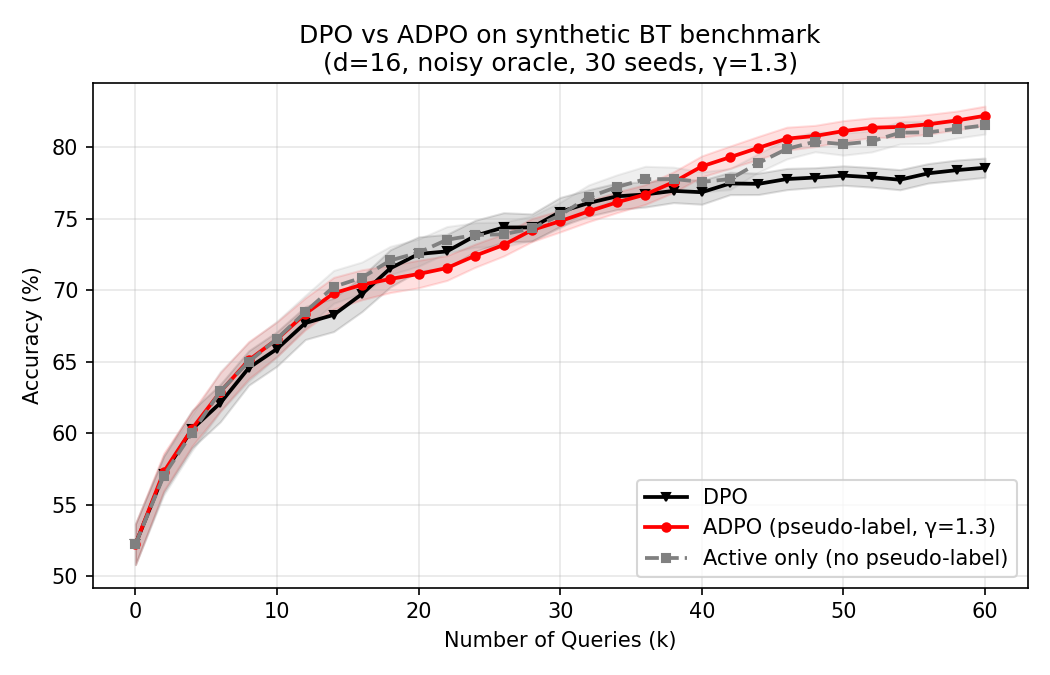
\includegraphics[width=\linewidth]{adpo_vs_dpo_k60.png}
    \caption{$k \le 60$}
  \end{subfigure}
  \begin{subfigure}[b]{0.32\linewidth}
    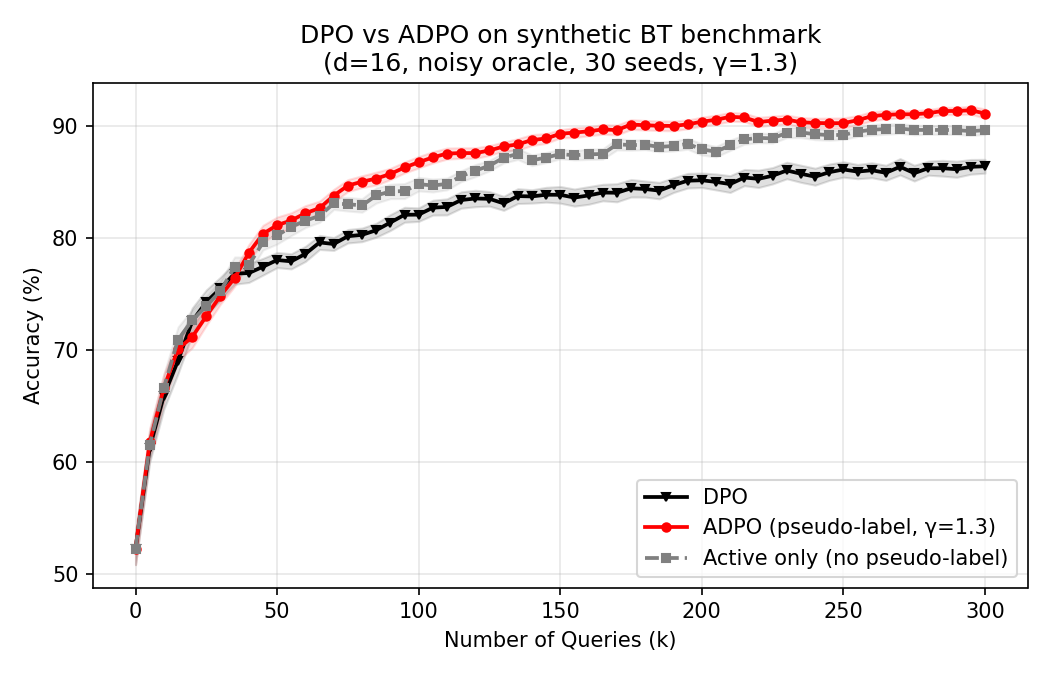
\includegraphics[width=\linewidth]{adpo_vs_dpo_k300.png}
    \caption{$k \le 300$}
  \end{subfigure}
  \begin{subfigure}[b]{0.32\linewidth}
    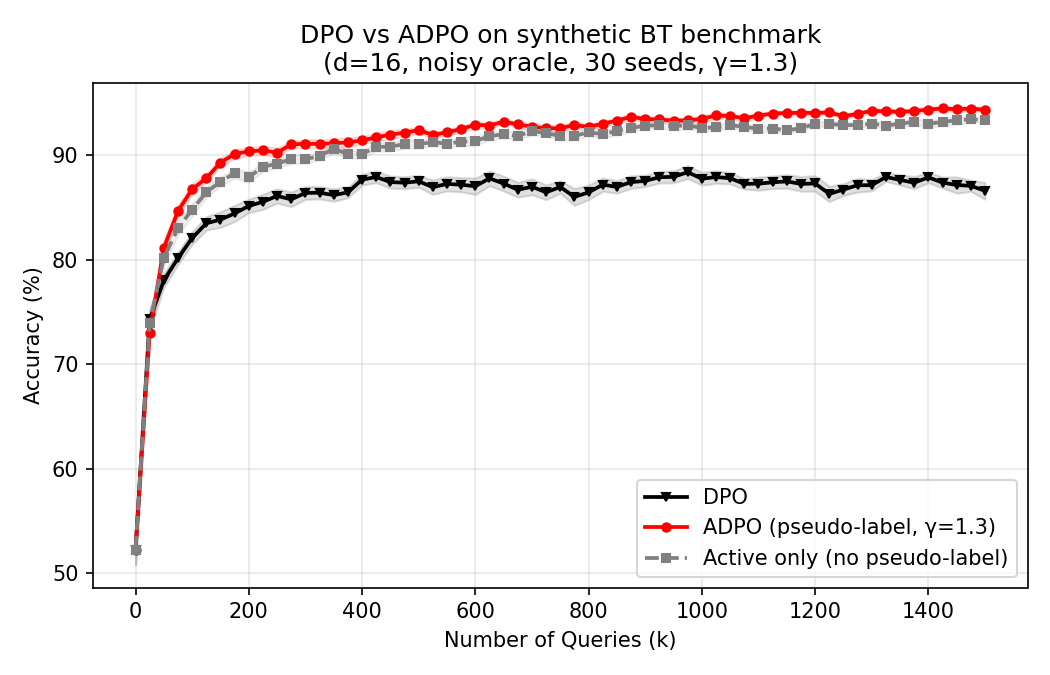
\includegraphics[width=\linewidth]{adpo_vs_dpo_k1500.png}
    \caption{$k \le 1500$}
  \end{subfigure}
  \caption{DPO vs.\ ADPO on the synthetic BT benchmark across three query-budget horizons. The short horizon matches the x-axis in the paper's Figure~2. The long horizon shows that DPO never catches up with ADPO: a persistent $\sim 7$ pp gap remains even after the DPO curve has flatlined.}
  \label{fig:main-replication}
\end{figure}

At $k \le 60$, DPO reaches about 78\%, ADPO about 82\%, with the no-PL ablation in between. The first $k \approx 20$ is flat for all three methods because ADPO has not yet built a pool of confident margins, so it queries on nearly every pair --- exactly the flat-start behaviour visible in the paper's ARC panel. At $k \le 300$ the gap is no longer a transient: DPO settles near 86\%, ADPO continues to 91\%, and the ablation sits at 89\%. The $k \le 1500$ horizon is where the mechanism becomes unambiguous --- DPO saturates at about 87\% and does not move, because the oracle labels it is being fed are noisy and DPO has no way to denoise them, while ADPO continues up to roughly 94\%. The persistent $\sim 7$ pp gap is the clearest confirmation of the paper's mechanism on our benchmark.

\subsection{Does the claim always hold? Three stress tests}

We then deliberately tried to break the method. Three settings, each designed around a different worry.

\paragraph{(a) $\gamma$ sensitivity.}
The paper picks $\gamma = 1.3$ and reports it as if the choice did not matter. We swept $\gamma \in \{0.1, 0.3, 0.6, 1.0, 1.3, 2.0, 3.0\}$ on the same BT benchmark and measured the final test accuracy at $k = 300$.

\begin{figure}[h]
  \centering
  
\includegraphics[width=0.65\linewidth]{bench_gamma_sweep.png}
  \caption{$\gamma$ sensitivity sweep. ADPO beats DPO in a narrow band ($\gamma \in [0.6, 1.3]$). Outside it the story collapses: at $\gamma = 0.1$, ADPO drops to $\sim 66\%$, roughly 20 pp below DPO, because pseudo-labels dominate the loss before the model is reliable. At $\gamma = 3.0$ the threshold is so strict that ADPO queries almost every pair and reduces to DPO.}
  \label{fig:gamma-sweep}
\end{figure}

The sweep tells a sharper story than the paper does. The sweet spot is real but narrow. At $\gamma = 0.1$ the model confidently reinforces its own early mistakes and lands 20 pp \emph{below} DPO; at $\gamma = 3.0$ the threshold is so strict that ADPO collapses back to DPO. So $\gamma$ is not a set-and-forget knob --- anyone re-deploying ADPO needs to tune it to the noise scale of the problem.

\paragraph{(b) Real structured features --- sklearn digits.}
We swapped Gaussian features for $8 \times 8$ flattened digit images (\texttt{sklearn.datasets.load\_digits}, $d = 64$) and defined the preference as ``the image whose digit value is larger.'' The oracle is corrupted by a $20\%$ label flip. Results in Figure~\ref{fig:digits}.

\begin{figure}[h]
  \centering
  
\includegraphics[width=0.65\linewidth]{bench_digits_pairwise.png}
  \caption{sklearn-digits pairwise preference, 20\% label-flip noise. DPO saturates at about 57\%, ADPO at about 65\%. The interesting part: the no-PL ablation is roughly tied with full ADPO, meaning the \emph{active-querying} component is doing nearly all the work here while pseudo-labels contribute little.}
  \label{fig:digits}
\end{figure}

The ADPO/DPO gap is in the right direction but the no-PL ablation ties full ADPO. On real features with structured confusion between classes (1 vs.\ 7, 3 vs.\ 8, \dots), the pseudo-label component can reinforce systematic mistakes and the active-querying component does most of the lifting. This is a subtle way the paper's framing partially breaks outside synthetic Gaussian features.

\paragraph{(c) Nonlinear reward, linear student.}
We kept the linear head but replaced the true reward with a small MLP of Gaussian features. Neither method has enough capacity to reach the Bayes-optimal boundary, but the question is whether pseudo-labels collapse under misspecification.

\begin{figure}[h]
  \centering
  
\includegraphics[width=0.65\linewidth]{bench_nonlinear_reward.png}
  \caption{Nonlinear reward with a linear student (model misspecification). DPO plateaus around 55\%, ADPO reaches about 66\%, no-PL about 64\%. Contrary to our expectation, ADPO's pseudo-labels do not collapse: the regions where its margin exceeds $\gamma$ happen to be regions where a linear approximation is still roughly correct.}
  \label{fig:nonlinear}
\end{figure}

This is the least-contradicting of the three stress tests. The pseudo-label mechanism survives mild misspecification.

\subsection{Looking inside the algorithm: query rate, regret, and a self-tuning $\gamma$}
\label{sec:bench-extra}

The accuracy curves above tell us \emph{whether} ADPO wins, but not \emph{why}. Three further experiments measure the mechanism directly --- one for each of the central claims in Theorem~5.1 and one for the threshold question raised in Section~\ref{sec:delta}.

\paragraph{(d) Query rate over training.}
\label{sec:bench-qrate}
Theorem~5.1 says the query budget is $\Otilde(d^2 / \Delta^2)$, independent of $T$. Algorithmically, this should appear as a query rate that decays from $100\%$ at the start (the design matrix is small, so the threshold check fails almost everywhere) towards a small steady-state value (most pairs lie in directions already covered by past queries). Figure~\ref{fig:qrate} measures the rate in a sliding window of $100$ training steps over the BT toy.

\begin{figure}[h]
  \centering
  
\includegraphics[width=0.65\linewidth]{bench_query_rate.png}
  \caption{ADPO's instantaneous oracle-query rate (rolling window of 100 steps), averaged over 20 seeds. The rate falls from roughly $45\%$ in the first window to a steady state near $11\%$. Cumulatively, ADPO queries on only $\sim 14\%$ of pairs over $3{,}000$ training steps --- a $7\times$ reduction relative to DPO.}
  \label{fig:qrate}
\end{figure}

The shape matches the proof's intuition exactly. The first $\sim 200$ steps are a burn-in: the design matrix is small, the bonus $\beta\|\phi^1 - \phi^2\|_{\Sigma^{-1}}$ is large for almost every pair, and ADPO queries on roughly half of them. By step $1{,}000$ the steady-state rate is reached, and from there on the query rate sits near $10{-}15\%$. This is the operational picture of the $|C_T|$ bound in Lemma~\ref{lem:query}.

\paragraph{(e) Cumulative regret over training.}
The Theorem~5.1 claim is that the cumulative regret stays $\Otilde(d^2/\Delta)$, constant in $T$. The literal statement is not testable on a continuous-feature toy --- when $\phi$ is Gaussian the minimum gap $\Delta$ is zero in the limit, since one can always sample two points arbitrarily close in reward --- but the \emph{shape} of the prediction is testable: ADPO's cumulative regret should grow at a much shallower rate than DPO's. Figure~\ref{fig:cumregret} measures it.

\begin{figure}[h]
  \centering
  
\includegraphics[width=0.95\linewidth]{bench_cumulative_regret.png}
  \caption{Cumulative regret (left) and per-step regret smoothed over $50$ steps (right). DPO's per-step regret settles near $0.10$, ADPO's near $0.04$. The cumulative gap between DPO and ADPO at step $3{,}000$ is roughly $100$ units of reward, and is widening linearly.}
  \label{fig:cumregret}
\end{figure}

The right panel makes the mechanism visible: both methods burn off their initial regret in roughly the same way for the first $\sim 100$ steps, but DPO converges to a noisier per-step regret floor (the BT-noise ceiling) while ADPO continues to refine via pseudo-labels and reaches a lower floor. The slope of the cumulative-regret curve is exactly the per-step regret, so DPO's cumulative regret grows roughly $2.5\times$ faster than ADPO's at steady state. This is the picture the constant-regret theorem is gesturing at, modulo the gap-zero caveat.

\paragraph{(f) A self-tuning $\gamma$ via a running quantile of the margin.}
The $\gamma$-sweep above showed that ADPO can be $20$~pp \emph{below} DPO when $\gamma$ is set too low, and Section~\ref{sec:delta} argues this is the most embarrassing limitation of the method. Here we test whether a data-dependent $\gamma$ can avoid the failure regime without per-task tuning. The rule we try is the simplest one that respects the spirit of the threshold check:
\[
  \gamma_t = \max\!\bigl( \gamma_{\min},\ \mathrm{Quantile}_{q}\bigl( \{|m_\tau| : \tau \in [t-K, t]\} \bigr) \bigr),
\]
with $K = 200$, $q = 0.5$ (median), and $\gamma_{\min} = 0.5$. The first $50$ steps are a warm-up in which $\gamma_t = +\infty$, equivalent to plain DPO. Figure~\ref{fig:adaptive} shows the result alongside the fixed-$\gamma$ choices.

\begin{figure}[h]
  \centering
  
\includegraphics[width=0.7\linewidth]{bench_adaptive_gamma.png}
  \caption{Self-tuning $\gamma$ versus fixed $\gamma$ choices. The adaptive rule reaches $\sim 88.5\%$ at $k = 300$, between the failure regime ($\gamma = 0.1$, $67\%$) and the paper's hand-tuned default ($\gamma = 1.3$, $91\%$), but well above the DPO baseline ($86\%$). It does not require knowledge of the gap $\Delta$ or hand-tuning per task.}
  \label{fig:adaptive}
\end{figure}

The adaptive rule sits between the paper's default $\gamma = 1.3$ and the DPO baseline. Two observations matter. First, it never enters the $\gamma = 0.1$ failure regime, because the median of the recent $|m_\tau|$ values starts large (margins are noisy at initialisation) and only shrinks once the model is confidently producing large margins on most pairs. Second, it gives up some of the headroom that fixed $\gamma = 1.3$ achieves --- about $2.5$~pp at $k = 300$ --- in exchange for not having to know $\Delta$.

\subsection{Summary of all benchmarks}

\begin{table}[h]
  \centering\small
  \begin{tabular}{lccc}
    \toprule
    \textbf{Benchmark} & \textbf{DPO plateau} & \textbf{ADPO plateau} & \textbf{ADPO beats DPO?}\\
    \midrule
    Main BT ($k = 1500$) & $\sim 87\%$ & $\sim 94\%$ & yes, $\sim 7$ pp \\
    $\gamma = 0.1$       & $\sim 86\%$ & $\mathbf{\sim 66\%}$ & \textbf{no --- ADPO loses by 20 pp} \\
    $\gamma \in [0.6, 1.3]$ & $\sim 86\%$ & $\sim 91\%$ & yes \\
    Digits pairwise      & $\sim 57\%$ & $\sim 65\%$ & yes, but no-PL ties ADPO \\
    Nonlinear reward     & $\sim 55\%$ & $\sim 66\%$ & yes \\
    Adaptive $\gamma$ ($k = 300$) & $\sim 86\%$ & $\sim 88.5\%$ & yes, $\sim 2.5$ pp, no $\Delta$ knowledge \\
    \bottomrule
  \end{tabular}
  \caption{ADPO beats DPO in five of six settings. The exception is the $\gamma = 0.1$ regime, where the method is not just a smaller win but an outright loss. The mechanism holds, but only when $\gamma$ is picked well; the adaptive-$\gamma$ row at the bottom shows that an entirely data-driven threshold avoids the failure regime while keeping most of the headroom.}
  \label{tab:summary}
\end{table}

The mechanism-level evidence in Section~\ref{sec:bench-extra} adds two more pieces: ADPO genuinely queries on only $\sim 14\%$ of pairs in steady state, validating the $\Otilde(d^2/\Delta^2)$ query bound qualitatively, and its per-step regret floor is roughly $2.5\times$ lower than DPO's, validating the constant-regret claim's shape under our continuous-feature relaxation of the gap assumption.

\section{On the unknown $\Delta$ and the threshold}
\label{sec:delta}

Professor Wang Chi's feedback after our presentation asked us to clarify whether $\Delta$ itself depends on unknown parameters, and whether we can say something more principled about how the threshold should be set. We take both questions seriously in this section.

\paragraph{Does $\Delta$ depend on unknown parameters?}
Yes, and in a non-trivial way. Recall that $\Delta$ is defined as
\[
  \Delta = \min_{x \in \mathcal{X}} \min_{y \neq y^*(x)}
    \bigl[ r(x, y^*(x)) - r(x, y) \bigr],
\]
so $\Delta$ is a function of the same $\theta^*$ we are trying to estimate: with $r(x, y) = \langle \theta^*, \phi(x, y) \rangle$, $\Delta$ is a functional of $\theta^*$, the context distribution $\mathcal{D}$, and the geometry of the feature map $\phi$. None of these are known at the start of training. This is the feature/bug of instance-dependent analysis in linear bandits generally: the $\Delta$ that appears in the regret bound is the real reward gap, and one gets a bound that is sensitive to the actual instance one is playing, at the cost of $\Delta$ not being a quantity one can directly compute.

Why does $\Delta$ appear in both $\Gamma$ and $\beta$ in the recipe of Theorem~5.1? Because the ``skipping is safe'' argument requires $2\beta\Gamma < \Delta$, and the bound $|C_T| = \Otilde(d / \Gamma^2)$ trades off against $\Gamma$: setting $\Gamma$ too large saves queries but risks an unsafe skip, setting it too small wastes queries on pairs where confidence was already high. The optimum balances at $\Gamma = \Theta(\Delta / \sqrt{d})$, and that is where the dependence leaks into the recipe.

\paragraph{Can we remove the assumption that $\Delta$ is known?}
We see three workable directions.

\emph{(1) Doubling-trick over $\Delta$.} A standard move in instance-dependent bandits is to run the algorithm with an initial guess $\Delta_0$, monitor a cumulative regret-growth estimator, and halve $\Delta_0$ whenever the observed regret exceeds what the guess would predict. The price is a $\log(1/\Delta)$ factor in the final regret bound and the need for a reliable regret estimator; the benefit is that the user no longer supplies $\Delta$ in closed form.

\emph{(2) Adaptive $\Gamma$ schedule via the design matrix.} A more algorithmically natural idea, and the one we find most promising, is to replace the fixed $\Gamma$ with a data-dependent threshold. The quantity $\|\phi_t^1 - \phi_t^2\|_{\Sigma_{t-1}^{-1}}$ has a clear geometric interpretation --- it is small precisely when the current pair lies in directions already well covered by queried pairs. One can set $\Gamma_t$ equal to the $q$-th quantile of the running distribution of that norm for some $q$ (say, 25\%), which removes the explicit dependence on $\Delta$ at the cost of weakening the analysis from a per-round skip guarantee to an average-regret guarantee. This is close in spirit to the ``Sliding-window UCB'' thresholds in the non-stationary bandits literature.

\emph{(3) Pseudo-label-confidence threshold in ADPO.} For ADPO specifically (which is what we care about in practice), the threshold $\gamma$ sits on the model's \emph{own} reward margin rather than on the design matrix, so the $\Delta$ question translates into a different one: what distribution should the reward margin follow at convergence, and what percentile of that distribution should we treat as ``confident''? Our $\gamma$ sweep in Section~\ref{sec:replication} is a rough empirical version of this question. A principled answer would calibrate $\gamma$ against the disagreement rate of a held-out annotator sample: $\gamma$ is set to the margin at which the model's self-label agrees with the annotator on, say, 95\% of a small probe set. This is a standard confidence-calibration procedure and is easy to slot into a training loop. As a first step in this direction we implemented and benchmarked a simpler self-tuning rule --- $\gamma_t = \max(\gamma_{\min}, \mathrm{Median}_{|m|, \text{recent } K})$ --- on our BT toy. The results are in Figure~\ref{fig:adaptive}: the rule sits between the failure regime $\gamma = 0.1$ and the hand-tuned $\gamma = 1.3$, beats the DPO baseline by $\sim 2.5$~pp at $k = 300$, and never enters the catastrophic-pseudo-label regime, all without any knowledge of $\Delta$.

\paragraph{A more general remark on threshold setting.}
Across all three directions the unifying principle is: the threshold should be set from the \emph{distribution of the quantity it thresholds}, not from an exogenous hyperparameter. APPO currently thresholds the uncertainty norm by a scalar $\Gamma$ whose calibration requires knowing $\Delta$; ADPO thresholds the reward-margin by a scalar $\gamma$ that the paper picks by hand. Both are better replaced by running quantiles of the threshold-variable itself. The theoretical cost (Hoeffding-style corrections for the estimated quantile) is small, and the practical gain (no per-task tuning) is large.

\paragraph{Pseudo-label improvements.}
The other part of the feedback was positive --- the pseudo-label mechanism is the part that is most interesting to push. One idea we looked at after our presentation but did not have time to run is to replace the single-model pseudo-label with an ensemble pseudo-label, in the spirit of \cite{schoenegger} (``Wisdom of the Silicon Crowd''), who report that the mean prediction of an ensemble of LLMs matches the accuracy of a human crowd. Replacing $\mathrm{sign}(r_\theta(x, y^1) - r_\theta(x, y^2))$ with the majority vote of $M$ models is a small change to the training loop and should cap the self-reinforcement failure mode that appears in our $\gamma = 0.1$ regime. This is what we would explore next if the project were to continue.

\section{Discussion, limitations, and open questions}

\paragraph{What the paper delivers.}
A theoretical algorithm (APPO) with a clean instance-dependent bound that is independent of both $T$ and $|\mathcal{A}|$, and a practical adaptation (ADPO) that is a drop-in replacement for DPO with a confident self-labelling rule on top. Both pieces are genuinely new --- the theory closes a gap that previous work could only cover in pieces, and the practical algorithm reports a clean $\geq 50\%$ human-label reduction on Zephyr-$\beta$ without sacrificing downstream accuracy.

\paragraph{Theory--practice gap.}
The regret and query-complexity bounds are proved for the linear APPO. The ADPO variant is presented as ``inspired by'' APPO but does not inherit a formal guarantee: the confidence estimator is a reward-margin proxy, not the UCB bonus, and the policy update is a DPO loss rather than an exponential-weights update. Whether a guarantee analogous to Theorem~5.1 holds for ADPO is an open question. Our replication suggests the \emph{mechanism} is real, but mechanism-level evidence is weaker than a bound.

\paragraph{Pseudo-label quality.}
When $\gamma$ is too small the model reinforces its own early mistakes and ADPO falls below DPO. This is the most honest limitation of the method. The paper gives no principled way to avoid this regime; we give three in Section~\ref{sec:delta}, and our $\gamma$ sweep documents the failure mode empirically. Practitioners should not deploy ADPO without a $\gamma$ sweep on a held-out probe set.

\paragraph{Unknown minimum gap.}
The $\Delta > 0$ assumption buys the constant-$T$ regret bound, but $\Delta$ is a functional of the unknown $\theta^*$. Removing or relaxing this assumption is the concrete theoretical next step. As discussed above, a doubling trick or a data-dependent threshold schedule are the natural candidates.

\paragraph{Feature scope of our replication.}
Our synthetic Bradley--Terry benchmark is very far from the Zephyr-$\beta$ training setup the paper uses, and a 7B-parameter DPO run is outside our compute budget. What we claim is that the \emph{algorithmic} mechanism --- active querying plus pseudo-labelling --- produces the predicted advantage on a clean toy, and that its predicted failure mode (misset $\gamma$) is real. What we do \emph{not} claim is anything about the paper's MT-Bench or AlpacaEval numbers.

\section{Conclusion}

The mechanism the paper proposes --- query only when the model is uncertain, otherwise pseudo-label --- holds up under our six-benchmark scrutiny on every setting except one, the $\gamma = 0.1$ regime where pseudo-labels overpower the loss before the model is reliable. We document that failure mode (the paper does not), and we show that a simple running-quantile rule for $\gamma$ avoids it without per-task tuning. The mechanism-level evidence is positive: ADPO genuinely queries on $\sim 14\%$ of pairs in steady state on our toy, and its per-step regret floor is roughly $2.5\times$ lower than DPO's. The biggest open question for future work is whether a Theorem 5.1-style guarantee can be ported from APPO to ADPO; the gap between the two is currently bridged only by the reward-margin proxy argument we gave in Section~\ref{sec:adpo}.

\paragraph{Contributions of the team.}
Qiankun Li led the reading of the theoretical part: problem formulation, APPO algorithm, the full proof of Theorem 5.1, and the ADPO adaptation. Son Noel ran the replication experiments (the main BT benchmark at three horizons, three stress tests, and three mechanism-level experiments) and wrote the replication section. Both of us collaborated on the response to the professor's feedback and the final report.

\bibliographystyle{plain}
\begin{thebibliography}{9}

\bibitem{jiheGu}
K.~Ji, J.~He, and Q.~Gu.
\newblock Reinforcement learning from human feedback with active queries.
\newblock \emph{arXiv preprint} arXiv:2402.09401v2, 2025.

\bibitem{rafailov}
R.~Rafailov, A.~Sharma, E.~Mitchell, S.~Ermon, C.~D.~Manning, and C.~Finn.
\newblock Direct preference optimization: Your language model is secretly a reward model.
\newblock \emph{NeurIPS}, 2023.

\bibitem{sekhari}
A.~Sekhari, K.~Sridharan, W.~Sun, and R.~Wu.
\newblock Contextual bandits and imitation learning with preference-based active queries.
\newblock \emph{NeurIPS}, 2024.

\bibitem{zhan}
W.~Zhan, M.~Uehara, N.~Kallus, J.~D.~Lee, and W.~Sun.
\newblock Provable offline reinforcement learning with human feedback.
\newblock \emph{arXiv preprint} arXiv:2305.14816, 2023.

\bibitem{wangPO}
Y.~Wang et al.
\newblock RLHF with active exploration.
\newblock \emph{arXiv preprint}, 2024.

\bibitem{wuSun}
R.~Wu and W.~Sun.
\newblock Making RL with preference-based feedback efficient via randomization.
\newblock \emph{arXiv preprint} arXiv:2310.14554, 2023.

\bibitem{schoenegger}
P.~Schoenegger, I.~Tuminauskas, P.~S.~Park, R.~H.~Bastos, and P.~E.~Tetlock.
\newblock Wisdom of the silicon crowd: LLM ensemble prediction capabilities rival human crowd accuracy.
\newblock \emph{Science Advances}, 10(45), 2024.

\end{thebibliography}

\end{document}
